\newpage
\blindtext[1]
\begin{figure}[H]
    \centering
    \begin{subfigure}[b]{\textwidth}
    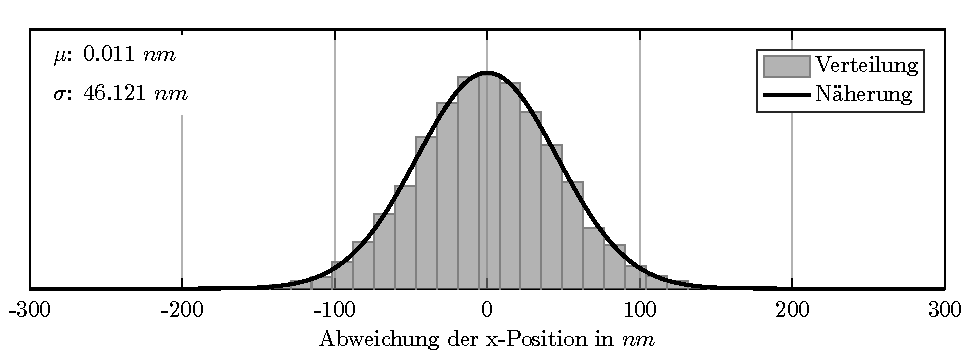
\includegraphics{graphics/results/drift/fig_drift_axis_tx.pdf}
    \end{subfigure}
    \begin{subfigure}[b]{\textwidth}
    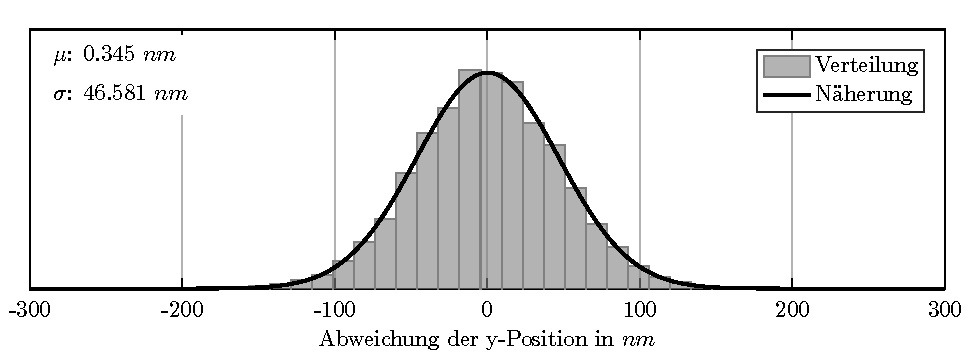
\includegraphics{graphics/results/drift/fig_drift_axis_ty.pdf}
    \end{subfigure}
    \begin{subfigure}[b]{\textwidth}
    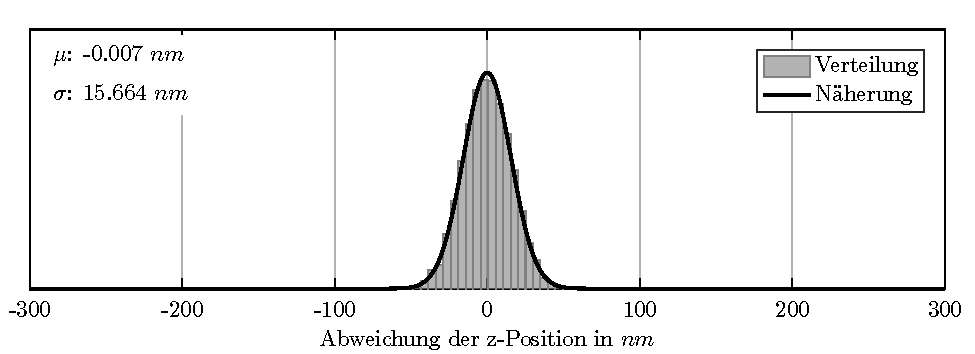
\includegraphics{graphics/results/drift/fig_drift_axis_tz.pdf}
    \end{subfigure}
    \caption[Abweichung der Plattformposition]{Abweichung der Plattformposition}\label{fig:results_drift_t}
\end{figure}
\blindtext[1]
\begin{figure}[H]
    \centering
    \begin{subfigure}[b]{\textwidth}
    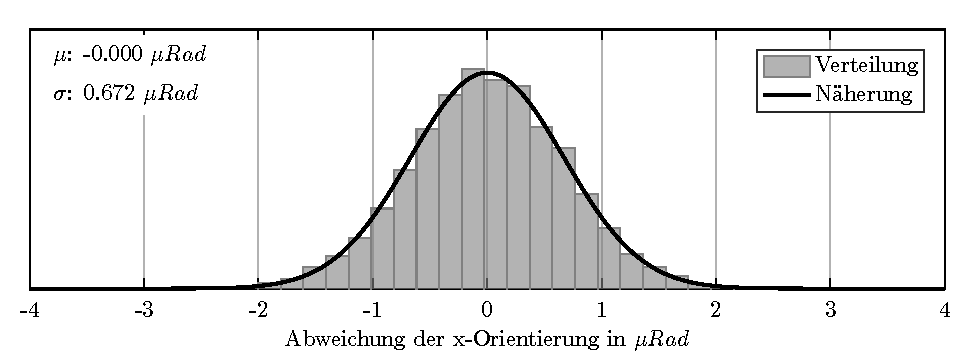
\includegraphics{graphics/results/drift/fig_drift_axis_rx.pdf}
    \end{subfigure}
    \begin{subfigure}[b]{\textwidth}
    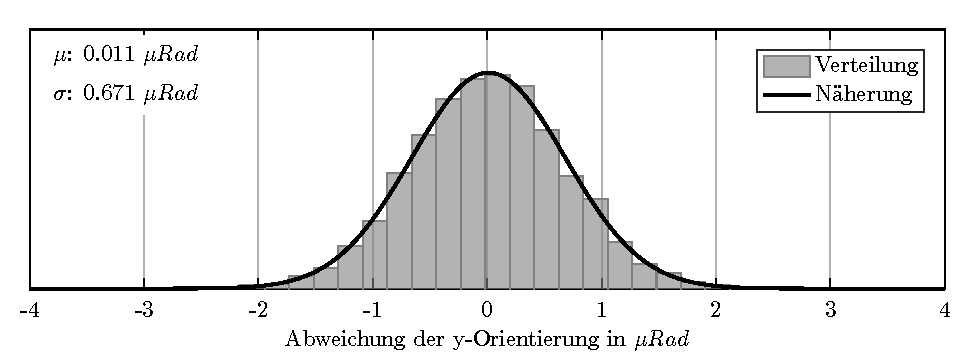
\includegraphics{graphics/results/drift/fig_drift_axis_ry.pdf}
    \end{subfigure}
    \begin{subfigure}[b]{\textwidth}
    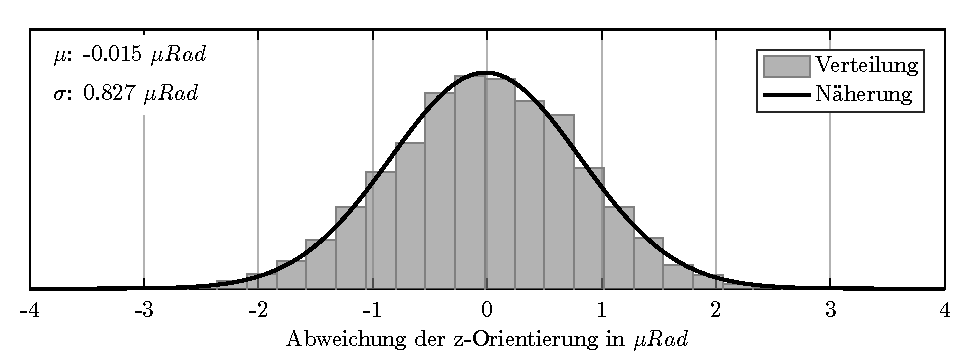
\includegraphics{graphics/results/drift/fig_drift_axis_rz.pdf}
    \end{subfigure}
    \caption[Abweichung der Plattformorientierung]{Abweichung der Plattformorientierung}\label{fig:results_drift_r}
\end{figure}
\blindtext[1]